% ============================================================
% Punkt 1: Wstęp teoretyczny
% Projekt układu sumatora pełnego (Full Adder)
% z minimalizacją bramek logicznych
% ------------------------------------------------------------
% Plik przeznaczony do włączenia w dokumencie głównym Overleaf:
%   % ============================================================
% Punkt 1: Wstęp teoretyczny
% Projekt układu sumatora pełnego (Full Adder)
% z minimalizacją bramek logicznych
% ------------------------------------------------------------
% Plik przeznaczony do włączenia w dokumencie głównym Overleaf:
%   % ============================================================
% Punkt 1: Wstęp teoretyczny
% Projekt układu sumatora pełnego (Full Adder)
% z minimalizacją bramek logicznych
% ------------------------------------------------------------
% Plik przeznaczony do włączenia w dokumencie głównym Overleaf:
%   % ============================================================
% Punkt 1: Wstęp teoretyczny
% Projekt układu sumatora pełnego (Full Adder)
% z minimalizacją bramek logicznych
% ------------------------------------------------------------
% Plik przeznaczony do włączenia w dokumencie głównym Overleaf:
%   \input{01_wstep_teoretyczny}
% Wymagane pakiety w dokumencie głównym:
%   \usepackage[utf8]{inputenc}  \usepackage[T1]{polski}
%   \usepackage{amsmath, amssymb}
% ============================================================

\section{Wstęp teoretyczny}

\subsection{Definicja sumatora cyfrowego}

Sumator cyfrowy jest układem kombinacyjnym służącym do wykonywania operacji arytmetycznego dodawania liczb zapisanych w postaci binarnej. Jego zadaniem jest wyznaczenie sumy wartości podanych na wejścia układu wraz z ewentualnym przeniesieniem powstającym podczas dodawania. W zależności od zastosowania sumator może operować na pojedynczych bitach lub na wielobitowych słowach danych.

W niniejszym projekcie analizowany jest sumator pełny (Full Adder), którego zadaniem jest dodanie trzech bitów: dwóch bitów argumentów oraz bitu przeniesienia z niższego rzędu. Układ posiada trzy wejścia binarne oraz dwa wyjścia informujące o wyniku dodawania.

Dla przyjętego rozwiązania:
\begin{equation*}
A = a_1a_0, \qquad B = b_1b_0,
\end{equation*}
gdzie $a_i$ są bitami pierwszej liczby, natomiast $b_i$ bitami drugiej liczby. W przypadku pojedynczej pozycji sumator pełny realizuje zależność:
\begin{equation*}
S = A + B + C_{in}.
\end{equation*}

Wyjście układu oznaczone jako $S$ (suma) przyjmuje wartość:
\begin{equation*}
S = 1
\end{equation*}
gdy:
\begin{equation*}
a \oplus b \oplus c_{in} = 1,
\end{equation*}
oraz:
\begin{equation*}
S = 0
\end{equation*}
gdy:
\begin{equation*}
a \oplus b \oplus c_{in} = 0.
\end{equation*}

Drugim wyjściem układu jest przeniesienie $C_{out}$, które przyjmuje wartość logiczną 1, gdy co najmniej dwa z trzech sygnałów wejściowych znajdują się w stanie wysokim.

Sumator pełny może być zrealizowany przy wykorzystaniu podstawowych bramek logicznych, takich jak AND, OR oraz NOT. Możliwe jest również wykorzystanie bramek XOR. W projekcie szczególną uwagę poświęcono minimalizacji liczby wykorzystanych bramek logicznych, dzięki czemu możliwe jest uzyskanie prostszego i bardziej efektywnego układu.

\subsection{Zasada działania sumatora pełnego}

Sumator pełny wykonuje dodawanie trzech bitów zgodnie z regułami arytmetyki binarnej. Podczas dodawania pojedynczych bitów może powstać dwucyfrowy wynik, którego starszy bit stanowi przeniesienie do następnej pozycji.

Dla dwóch bitów $a$ i $b$ możliwe są następujące przypadki:
\begin{align*}
0 + 0 &= 00, \\
0 + 1 &= 01, \\
1 + 0 &= 01, \\
1 + 1 &= 10.
\end{align*}

Sumator pełny uwzględnia dodatkowo trzeci składnik, którym jest przeniesienie $c_{in}$ otrzymane z niższego rzędu. Dodawanie trzech bitów może więc wytworzyć wynik dwucyfrowy o postaci $c_{out}s$, gdzie $s$ jest bitem sumy, a $c_{out}$ przeniesieniem do rzędu wyższego.

Działanie układu można opisać za pomocą następujących zależności. Suma bitów wyraża się wzorem:
\begin{equation*}
s = a \oplus b \oplus c_{in},
\end{equation*}
natomiast przeniesienie wynosi:
\begin{equation*}
c_{out} = a \cdot b \vee c_{in} \cdot (a \oplus b).
\end{equation*}

Wprowadzając oznaczenie pomocnicze:
\begin{equation*}
c_1 = a \oplus b,
\end{equation*}
działanie układu można przedstawić jako dwa etapy:
\begin{equation*}
c_1 = a \oplus b, \qquad s = c_1 \oplus c_{in}, \qquad c_{out} = a \cdot b \vee c_1 \cdot c_{in}.
\end{equation*}

Dzięki temu wyjście $s$ będzie równe 1 wyłącznie wtedy, gdy nieparzysta liczba sygnałów wejściowych przyjmuje wartość logiczną 1, natomiast przeniesienie $c_{out}$ pojawi się w sytuacji, gdy wartość sumy argumentów przekroczy pojemność pojedynczego bitu.

Symbol blokowy sumatora pełnego przedstawia Rysunek~\ref{fig:symbol-fa}.

\begin{figure}[h]
    \centering
    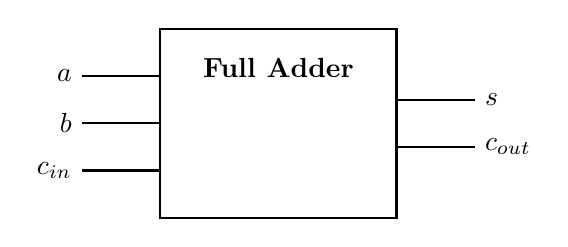
\begin{tikzpicture}
        \draw[thick] (0,0) rectangle (3,2.4);
        \node at (1.5,1.9) {\textbf{Full Adder}};
        \draw[thick] (-1,1.8) -- (0,1.8) node[midway, above] {};
        \node[left] at (-1,1.8) {$a$};
        \draw[thick] (-1,1.2) -- (0,1.2);
        \node[left] at (-1,1.2) {$b$};
        \draw[thick] (-1,0.6) -- (0,0.6);
        \node[left] at (-1,0.6) {$c_{in}$};
        \draw[thick] (3,1.5) -- (4,1.5);
        \node[right] at (4,1.5) {$s$};
        \draw[thick] (3,0.9) -- (4,0.9);
        \node[right] at (4,0.9) {$c_{out}$};
    \end{tikzpicture}
    \caption{Symbol blokowy sumatora pełnego (Full Adder)}
    \label{fig:symbol-fa}
\end{figure}

\subsection{Zastosowanie sumatorów cyfrowych}

Sumatory cyfrowe są powszechnie stosowane w układach cyfrowych, w których konieczne jest wykonywanie operacji arytmetycznych na wartościach binarnych.

Przykładowe zastosowania sumatorów obejmują:
\begin{itemize}
    \item procesory i jednostki arytmetyczno-logiczne (ALU),
    \item układy dodawania liczb wielobitowych,
    \item układy mnożenia i dzielenia binarnego,
    \item liczniki i układy inkrementacji wartości,
    \item układy adresowania pamięci,
    \item cyfrowe przetwarzanie sygnałów (DSP),
    \item układy korekcji kodu BCD,
    \item systemy mikroprocesorowe i mikrokontrolerowe.
\end{itemize}

Sumator pełny może być wykorzystany między innymi do realizacji jednej pozycji dodawania liczb wielobitowych. Przykładowo, układ może stanowić pojedyncze ogniwo kaskady sumującej liczby o dowolnej długości słowa.

W większych systemach sumatory pełne są łączone ze sobą w celu realizacji dodawania liczb o większej liczbie bitów, przy czym przeniesienie z każdego rzędu podawane jest na wejście rzędu wyższego.

\subsection{Rodzaje sumatorów}

Sumatory cyfrowe można podzielić ze względu na liczbę obsługiwanych argumentów oraz sposób przekazywania przeniesienia. Najczęściej wyróżnia się trzy podstawowe typy:
\begin{itemize}
    \item Półsumator (Half Adder) -- dodaje dwa bity $a$ i $b$, wyznaczając sumę $s = a \oplus b$ oraz przeniesienie $c = a \cdot b$; nie posiada wejścia przeniesienia z niższego rzędu.
    \item Sumator pełny (Full Adder) -- dodaje trzy bity $a$, $b$ oraz $c_{in}$, wyznaczając sumę oraz przeniesienie do rzędu wyższego; stanowi podstawowy element układów sumujących wielobitowych.
    \item Sumator kaskadowy (Ripple-Carry Adder) -- powstaje przez połączenie kaskadowe sumatorów pełnych, w którym przeniesienie z każdego rzędu podawane jest na wejście przeniesienia rzędu następnego.
\end{itemize}

W praktycznych układach wyróżnia się również bardziej zaawansowane struktury, takie jak sumatory z przyspieszonym przeniesieniem (Carry-Lookahead Adder), w których przeniesienia wyznaczane są równolegle dla wszystkich pozycji, co pozwala zredukować czas propagacji sygnału kosztem zwiększenia złożoności układu.

Ze względu na liczbę bitów obsługiwanych przez pojedynczy stopień można wyróżnić sumatory jedno- oraz wielobitowe. Zwiększenie liczby bitów powoduje wzrost złożoności układu, dlatego istotnym elementem projektowania układów cyfrowych jest ich odpowiednia minimalizacja.

W niniejszym projekcie zastosowany zostanie pojedynczy sumator pełny. Układ będzie dodawał trzy bity wejściowe $a$, $b$ oraz $c_{in}$, a jego wyjścia $s$ oraz $c_{out}$ będą informowały o wartości sumy oraz przeniesienia. Następnie układ zostanie poddany procesowi minimalizacji w celu ograniczenia liczby wymaganych bramek logicznych.

% Wymagane pakiety w dokumencie głównym:
%   \usepackage[utf8]{inputenc}  \usepackage[T1]{polski}
%   \usepackage{amsmath, amssymb}
% ============================================================

\section{Wstęp teoretyczny}

\subsection{Definicja sumatora cyfrowego}

Sumator cyfrowy jest układem kombinacyjnym służącym do wykonywania operacji arytmetycznego dodawania liczb zapisanych w postaci binarnej. Jego zadaniem jest wyznaczenie sumy wartości podanych na wejścia układu wraz z ewentualnym przeniesieniem powstającym podczas dodawania. W zależności od zastosowania sumator może operować na pojedynczych bitach lub na wielobitowych słowach danych.

W niniejszym projekcie analizowany jest sumator pełny (Full Adder), którego zadaniem jest dodanie trzech bitów: dwóch bitów argumentów oraz bitu przeniesienia z niższego rzędu. Układ posiada trzy wejścia binarne oraz dwa wyjścia informujące o wyniku dodawania.

Dla przyjętego rozwiązania:
\begin{equation*}
A = a_1a_0, \qquad B = b_1b_0,
\end{equation*}
gdzie $a_i$ są bitami pierwszej liczby, natomiast $b_i$ bitami drugiej liczby. W przypadku pojedynczej pozycji sumator pełny realizuje zależność:
\begin{equation*}
S = A + B + C_{in}.
\end{equation*}

Wyjście układu oznaczone jako $S$ (suma) przyjmuje wartość:
\begin{equation*}
S = 1
\end{equation*}
gdy:
\begin{equation*}
a \oplus b \oplus c_{in} = 1,
\end{equation*}
oraz:
\begin{equation*}
S = 0
\end{equation*}
gdy:
\begin{equation*}
a \oplus b \oplus c_{in} = 0.
\end{equation*}

Drugim wyjściem układu jest przeniesienie $C_{out}$, które przyjmuje wartość logiczną 1, gdy co najmniej dwa z trzech sygnałów wejściowych znajdują się w stanie wysokim.

Sumator pełny może być zrealizowany przy wykorzystaniu podstawowych bramek logicznych, takich jak AND, OR oraz NOT. Możliwe jest również wykorzystanie bramek XOR. W projekcie szczególną uwagę poświęcono minimalizacji liczby wykorzystanych bramek logicznych, dzięki czemu możliwe jest uzyskanie prostszego i bardziej efektywnego układu.

\subsection{Zasada działania sumatora pełnego}

Sumator pełny wykonuje dodawanie trzech bitów zgodnie z regułami arytmetyki binarnej. Podczas dodawania pojedynczych bitów może powstać dwucyfrowy wynik, którego starszy bit stanowi przeniesienie do następnej pozycji.

Dla dwóch bitów $a$ i $b$ możliwe są następujące przypadki:
\begin{align*}
0 + 0 &= 00, \\
0 + 1 &= 01, \\
1 + 0 &= 01, \\
1 + 1 &= 10.
\end{align*}

Sumator pełny uwzględnia dodatkowo trzeci składnik, którym jest przeniesienie $c_{in}$ otrzymane z niższego rzędu. Dodawanie trzech bitów może więc wytworzyć wynik dwucyfrowy o postaci $c_{out}s$, gdzie $s$ jest bitem sumy, a $c_{out}$ przeniesieniem do rzędu wyższego.

Działanie układu można opisać za pomocą następujących zależności. Suma bitów wyraża się wzorem:
\begin{equation*}
s = a \oplus b \oplus c_{in},
\end{equation*}
natomiast przeniesienie wynosi:
\begin{equation*}
c_{out} = a \cdot b \vee c_{in} \cdot (a \oplus b).
\end{equation*}

Wprowadzając oznaczenie pomocnicze:
\begin{equation*}
c_1 = a \oplus b,
\end{equation*}
działanie układu można przedstawić jako dwa etapy:
\begin{equation*}
c_1 = a \oplus b, \qquad s = c_1 \oplus c_{in}, \qquad c_{out} = a \cdot b \vee c_1 \cdot c_{in}.
\end{equation*}

Dzięki temu wyjście $s$ będzie równe 1 wyłącznie wtedy, gdy nieparzysta liczba sygnałów wejściowych przyjmuje wartość logiczną 1, natomiast przeniesienie $c_{out}$ pojawi się w sytuacji, gdy wartość sumy argumentów przekroczy pojemność pojedynczego bitu.

Symbol blokowy sumatora pełnego przedstawia Rysunek~\ref{fig:symbol-fa}.

\begin{figure}[h]
    \centering
    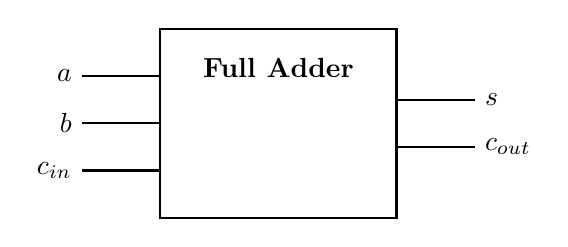
\begin{tikzpicture}
        \draw[thick] (0,0) rectangle (3,2.4);
        \node at (1.5,1.9) {\textbf{Full Adder}};
        \draw[thick] (-1,1.8) -- (0,1.8) node[midway, above] {};
        \node[left] at (-1,1.8) {$a$};
        \draw[thick] (-1,1.2) -- (0,1.2);
        \node[left] at (-1,1.2) {$b$};
        \draw[thick] (-1,0.6) -- (0,0.6);
        \node[left] at (-1,0.6) {$c_{in}$};
        \draw[thick] (3,1.5) -- (4,1.5);
        \node[right] at (4,1.5) {$s$};
        \draw[thick] (3,0.9) -- (4,0.9);
        \node[right] at (4,0.9) {$c_{out}$};
    \end{tikzpicture}
    \caption{Symbol blokowy sumatora pełnego (Full Adder)}
    \label{fig:symbol-fa}
\end{figure}

\subsection{Zastosowanie sumatorów cyfrowych}

Sumatory cyfrowe są powszechnie stosowane w układach cyfrowych, w których konieczne jest wykonywanie operacji arytmetycznych na wartościach binarnych.

Przykładowe zastosowania sumatorów obejmują:
\begin{itemize}
    \item procesory i jednostki arytmetyczno-logiczne (ALU),
    \item układy dodawania liczb wielobitowych,
    \item układy mnożenia i dzielenia binarnego,
    \item liczniki i układy inkrementacji wartości,
    \item układy adresowania pamięci,
    \item cyfrowe przetwarzanie sygnałów (DSP),
    \item układy korekcji kodu BCD,
    \item systemy mikroprocesorowe i mikrokontrolerowe.
\end{itemize}

Sumator pełny może być wykorzystany między innymi do realizacji jednej pozycji dodawania liczb wielobitowych. Przykładowo, układ może stanowić pojedyncze ogniwo kaskady sumującej liczby o dowolnej długości słowa.

W większych systemach sumatory pełne są łączone ze sobą w celu realizacji dodawania liczb o większej liczbie bitów, przy czym przeniesienie z każdego rzędu podawane jest na wejście rzędu wyższego.

\subsection{Rodzaje sumatorów}

Sumatory cyfrowe można podzielić ze względu na liczbę obsługiwanych argumentów oraz sposób przekazywania przeniesienia. Najczęściej wyróżnia się trzy podstawowe typy:
\begin{itemize}
    \item Półsumator (Half Adder) -- dodaje dwa bity $a$ i $b$, wyznaczając sumę $s = a \oplus b$ oraz przeniesienie $c = a \cdot b$; nie posiada wejścia przeniesienia z niższego rzędu.
    \item Sumator pełny (Full Adder) -- dodaje trzy bity $a$, $b$ oraz $c_{in}$, wyznaczając sumę oraz przeniesienie do rzędu wyższego; stanowi podstawowy element układów sumujących wielobitowych.
    \item Sumator kaskadowy (Ripple-Carry Adder) -- powstaje przez połączenie kaskadowe sumatorów pełnych, w którym przeniesienie z każdego rzędu podawane jest na wejście przeniesienia rzędu następnego.
\end{itemize}

W praktycznych układach wyróżnia się również bardziej zaawansowane struktury, takie jak sumatory z przyspieszonym przeniesieniem (Carry-Lookahead Adder), w których przeniesienia wyznaczane są równolegle dla wszystkich pozycji, co pozwala zredukować czas propagacji sygnału kosztem zwiększenia złożoności układu.

Ze względu na liczbę bitów obsługiwanych przez pojedynczy stopień można wyróżnić sumatory jedno- oraz wielobitowe. Zwiększenie liczby bitów powoduje wzrost złożoności układu, dlatego istotnym elementem projektowania układów cyfrowych jest ich odpowiednia minimalizacja.

W niniejszym projekcie zastosowany zostanie pojedynczy sumator pełny. Układ będzie dodawał trzy bity wejściowe $a$, $b$ oraz $c_{in}$, a jego wyjścia $s$ oraz $c_{out}$ będą informowały o wartości sumy oraz przeniesienia. Następnie układ zostanie poddany procesowi minimalizacji w celu ograniczenia liczby wymaganych bramek logicznych.

% Wymagane pakiety w dokumencie głównym:
%   \usepackage[utf8]{inputenc}  \usepackage[T1]{polski}
%   \usepackage{amsmath, amssymb}
% ============================================================

\section{Wstęp teoretyczny}

\subsection{Definicja sumatora cyfrowego}

Sumator cyfrowy jest układem kombinacyjnym służącym do wykonywania operacji arytmetycznego dodawania liczb zapisanych w postaci binarnej. Jego zadaniem jest wyznaczenie sumy wartości podanych na wejścia układu wraz z ewentualnym przeniesieniem powstającym podczas dodawania. W zależności od zastosowania sumator może operować na pojedynczych bitach lub na wielobitowych słowach danych.

W niniejszym projekcie analizowany jest sumator pełny (Full Adder), którego zadaniem jest dodanie trzech bitów: dwóch bitów argumentów oraz bitu przeniesienia z niższego rzędu. Układ posiada trzy wejścia binarne oraz dwa wyjścia informujące o wyniku dodawania.

Dla przyjętego rozwiązania:
\begin{equation*}
A = a_1a_0, \qquad B = b_1b_0,
\end{equation*}
gdzie $a_i$ są bitami pierwszej liczby, natomiast $b_i$ bitami drugiej liczby. W przypadku pojedynczej pozycji sumator pełny realizuje zależność:
\begin{equation*}
S = A + B + C_{in}.
\end{equation*}

Wyjście układu oznaczone jako $S$ (suma) przyjmuje wartość:
\begin{equation*}
S = 1
\end{equation*}
gdy:
\begin{equation*}
a \oplus b \oplus c_{in} = 1,
\end{equation*}
oraz:
\begin{equation*}
S = 0
\end{equation*}
gdy:
\begin{equation*}
a \oplus b \oplus c_{in} = 0.
\end{equation*}

Drugim wyjściem układu jest przeniesienie $C_{out}$, które przyjmuje wartość logiczną 1, gdy co najmniej dwa z trzech sygnałów wejściowych znajdują się w stanie wysokim.

Sumator pełny może być zrealizowany przy wykorzystaniu podstawowych bramek logicznych, takich jak AND, OR oraz NOT. Możliwe jest również wykorzystanie bramek XOR. W projekcie szczególną uwagę poświęcono minimalizacji liczby wykorzystanych bramek logicznych, dzięki czemu możliwe jest uzyskanie prostszego i bardziej efektywnego układu.

\subsection{Zasada działania sumatora pełnego}

Sumator pełny wykonuje dodawanie trzech bitów zgodnie z regułami arytmetyki binarnej. Podczas dodawania pojedynczych bitów może powstać dwucyfrowy wynik, którego starszy bit stanowi przeniesienie do następnej pozycji.

Dla dwóch bitów $a$ i $b$ możliwe są następujące przypadki:
\begin{align*}
0 + 0 &= 00, \\
0 + 1 &= 01, \\
1 + 0 &= 01, \\
1 + 1 &= 10.
\end{align*}

Sumator pełny uwzględnia dodatkowo trzeci składnik, którym jest przeniesienie $c_{in}$ otrzymane z niższego rzędu. Dodawanie trzech bitów może więc wytworzyć wynik dwucyfrowy o postaci $c_{out}s$, gdzie $s$ jest bitem sumy, a $c_{out}$ przeniesieniem do rzędu wyższego.

Działanie układu można opisać za pomocą następujących zależności. Suma bitów wyraża się wzorem:
\begin{equation*}
s = a \oplus b \oplus c_{in},
\end{equation*}
natomiast przeniesienie wynosi:
\begin{equation*}
c_{out} = a \cdot b \vee c_{in} \cdot (a \oplus b).
\end{equation*}

Wprowadzając oznaczenie pomocnicze:
\begin{equation*}
c_1 = a \oplus b,
\end{equation*}
działanie układu można przedstawić jako dwa etapy:
\begin{equation*}
c_1 = a \oplus b, \qquad s = c_1 \oplus c_{in}, \qquad c_{out} = a \cdot b \vee c_1 \cdot c_{in}.
\end{equation*}

Dzięki temu wyjście $s$ będzie równe 1 wyłącznie wtedy, gdy nieparzysta liczba sygnałów wejściowych przyjmuje wartość logiczną 1, natomiast przeniesienie $c_{out}$ pojawi się w sytuacji, gdy wartość sumy argumentów przekroczy pojemność pojedynczego bitu.

Symbol blokowy sumatora pełnego przedstawia Rysunek~\ref{fig:symbol-fa}.

\begin{figure}[h]
    \centering
    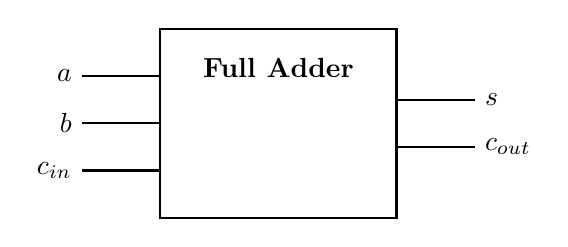
\begin{tikzpicture}
        \draw[thick] (0,0) rectangle (3,2.4);
        \node at (1.5,1.9) {\textbf{Full Adder}};
        \draw[thick] (-1,1.8) -- (0,1.8) node[midway, above] {};
        \node[left] at (-1,1.8) {$a$};
        \draw[thick] (-1,1.2) -- (0,1.2);
        \node[left] at (-1,1.2) {$b$};
        \draw[thick] (-1,0.6) -- (0,0.6);
        \node[left] at (-1,0.6) {$c_{in}$};
        \draw[thick] (3,1.5) -- (4,1.5);
        \node[right] at (4,1.5) {$s$};
        \draw[thick] (3,0.9) -- (4,0.9);
        \node[right] at (4,0.9) {$c_{out}$};
    \end{tikzpicture}
    \caption{Symbol blokowy sumatora pełnego (Full Adder)}
    \label{fig:symbol-fa}
\end{figure}

\subsection{Zastosowanie sumatorów cyfrowych}

Sumatory cyfrowe są powszechnie stosowane w układach cyfrowych, w których konieczne jest wykonywanie operacji arytmetycznych na wartościach binarnych.

Przykładowe zastosowania sumatorów obejmują:
\begin{itemize}
    \item procesory i jednostki arytmetyczno-logiczne (ALU),
    \item układy dodawania liczb wielobitowych,
    \item układy mnożenia i dzielenia binarnego,
    \item liczniki i układy inkrementacji wartości,
    \item układy adresowania pamięci,
    \item cyfrowe przetwarzanie sygnałów (DSP),
    \item układy korekcji kodu BCD,
    \item systemy mikroprocesorowe i mikrokontrolerowe.
\end{itemize}

Sumator pełny może być wykorzystany między innymi do realizacji jednej pozycji dodawania liczb wielobitowych. Przykładowo, układ może stanowić pojedyncze ogniwo kaskady sumującej liczby o dowolnej długości słowa.

W większych systemach sumatory pełne są łączone ze sobą w celu realizacji dodawania liczb o większej liczbie bitów, przy czym przeniesienie z każdego rzędu podawane jest na wejście rzędu wyższego.

\subsection{Rodzaje sumatorów}

Sumatory cyfrowe można podzielić ze względu na liczbę obsługiwanych argumentów oraz sposób przekazywania przeniesienia. Najczęściej wyróżnia się trzy podstawowe typy:
\begin{itemize}
    \item Półsumator (Half Adder) -- dodaje dwa bity $a$ i $b$, wyznaczając sumę $s = a \oplus b$ oraz przeniesienie $c = a \cdot b$; nie posiada wejścia przeniesienia z niższego rzędu.
    \item Sumator pełny (Full Adder) -- dodaje trzy bity $a$, $b$ oraz $c_{in}$, wyznaczając sumę oraz przeniesienie do rzędu wyższego; stanowi podstawowy element układów sumujących wielobitowych.
    \item Sumator kaskadowy (Ripple-Carry Adder) -- powstaje przez połączenie kaskadowe sumatorów pełnych, w którym przeniesienie z każdego rzędu podawane jest na wejście przeniesienia rzędu następnego.
\end{itemize}

W praktycznych układach wyróżnia się również bardziej zaawansowane struktury, takie jak sumatory z przyspieszonym przeniesieniem (Carry-Lookahead Adder), w których przeniesienia wyznaczane są równolegle dla wszystkich pozycji, co pozwala zredukować czas propagacji sygnału kosztem zwiększenia złożoności układu.

Ze względu na liczbę bitów obsługiwanych przez pojedynczy stopień można wyróżnić sumatory jedno- oraz wielobitowe. Zwiększenie liczby bitów powoduje wzrost złożoności układu, dlatego istotnym elementem projektowania układów cyfrowych jest ich odpowiednia minimalizacja.

W niniejszym projekcie zastosowany zostanie pojedynczy sumator pełny. Układ będzie dodawał trzy bity wejściowe $a$, $b$ oraz $c_{in}$, a jego wyjścia $s$ oraz $c_{out}$ będą informowały o wartości sumy oraz przeniesienia. Następnie układ zostanie poddany procesowi minimalizacji w celu ograniczenia liczby wymaganych bramek logicznych.

% Wymagane pakiety w dokumencie głównym:
%   \usepackage[utf8]{inputenc}  \usepackage[T1]{polski}
%   \usepackage{amsmath, amssymb}
% ============================================================

\section{Wstęp teoretyczny}

\subsection{Definicja sumatora cyfrowego}

Sumator cyfrowy jest układem kombinacyjnym służącym do wykonywania operacji arytmetycznego dodawania liczb zapisanych w postaci binarnej. Jego zadaniem jest wyznaczenie sumy wartości podanych na wejścia układu wraz z ewentualnym przeniesieniem powstającym podczas dodawania. W zależności od zastosowania sumator może operować na pojedynczych bitach lub na wielobitowych słowach danych.

W niniejszym projekcie analizowany jest sumator pełny (Full Adder), którego zadaniem jest dodanie trzech bitów: dwóch bitów argumentów oraz bitu przeniesienia z niższego rzędu. Układ posiada trzy wejścia binarne oraz dwa wyjścia informujące o wyniku dodawania.

Dla przyjętego rozwiązania:
\begin{equation*}
A = a_1a_0, \qquad B = b_1b_0,
\end{equation*}
gdzie $a_i$ są bitami pierwszej liczby, natomiast $b_i$ bitami drugiej liczby. W przypadku pojedynczej pozycji sumator pełny realizuje zależność:
\begin{equation*}
S = A + B + C_{in}.
\end{equation*}

Wyjście układu oznaczone jako $S$ (suma) przyjmuje wartość:
\begin{equation*}
S = 1
\end{equation*}
gdy:
\begin{equation*}
a \oplus b \oplus c_{in} = 1,
\end{equation*}
oraz:
\begin{equation*}
S = 0
\end{equation*}
gdy:
\begin{equation*}
a \oplus b \oplus c_{in} = 0.
\end{equation*}

Drugim wyjściem układu jest przeniesienie $C_{out}$, które przyjmuje wartość logiczną 1, gdy co najmniej dwa z trzech sygnałów wejściowych znajdują się w stanie wysokim.

Sumator pełny może być zrealizowany przy wykorzystaniu podstawowych bramek logicznych, takich jak AND, OR oraz NOT. Możliwe jest również wykorzystanie bramek XOR. W projekcie szczególną uwagę poświęcono minimalizacji liczby wykorzystanych bramek logicznych, dzięki czemu możliwe jest uzyskanie prostszego i bardziej efektywnego układu.

\subsection{Zasada działania sumatora pełnego}

Sumator pełny wykonuje dodawanie trzech bitów zgodnie z regułami arytmetyki binarnej. Podczas dodawania pojedynczych bitów może powstać dwucyfrowy wynik, którego starszy bit stanowi przeniesienie do następnej pozycji.

Dla dwóch bitów $a$ i $b$ możliwe są następujące przypadki:
\begin{align*}
0 + 0 &= 00, \\
0 + 1 &= 01, \\
1 + 0 &= 01, \\
1 + 1 &= 10.
\end{align*}

Sumator pełny uwzględnia dodatkowo trzeci składnik, którym jest przeniesienie $c_{in}$ otrzymane z niższego rzędu. Dodawanie trzech bitów może więc wytworzyć wynik dwucyfrowy o postaci $c_{out}s$, gdzie $s$ jest bitem sumy, a $c_{out}$ przeniesieniem do rzędu wyższego.

Działanie układu można opisać za pomocą następujących zależności. Suma bitów wyraża się wzorem:
\begin{equation*}
s = a \oplus b \oplus c_{in},
\end{equation*}
natomiast przeniesienie wynosi:
\begin{equation*}
c_{out} = a \cdot b \vee c_{in} \cdot (a \oplus b).
\end{equation*}

Wprowadzając oznaczenie pomocnicze:
\begin{equation*}
c_1 = a \oplus b,
\end{equation*}
działanie układu można przedstawić jako dwa etapy:
\begin{equation*}
c_1 = a \oplus b, \qquad s = c_1 \oplus c_{in}, \qquad c_{out} = a \cdot b \vee c_1 \cdot c_{in}.
\end{equation*}

Dzięki temu wyjście $s$ będzie równe 1 wyłącznie wtedy, gdy nieparzysta liczba sygnałów wejściowych przyjmuje wartość logiczną 1, natomiast przeniesienie $c_{out}$ pojawi się w sytuacji, gdy wartość sumy argumentów przekroczy pojemność pojedynczego bitu.

Symbol blokowy sumatora pełnego przedstawia Rysunek~\ref{fig:symbol-fa}.

\begin{figure}[h]
    \centering
    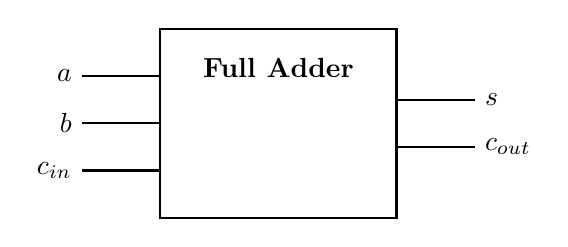
\begin{tikzpicture}
        \draw[thick] (0,0) rectangle (3,2.4);
        \node at (1.5,1.9) {\textbf{Full Adder}};
        \draw[thick] (-1,1.8) -- (0,1.8) node[midway, above] {};
        \node[left] at (-1,1.8) {$a$};
        \draw[thick] (-1,1.2) -- (0,1.2);
        \node[left] at (-1,1.2) {$b$};
        \draw[thick] (-1,0.6) -- (0,0.6);
        \node[left] at (-1,0.6) {$c_{in}$};
        \draw[thick] (3,1.5) -- (4,1.5);
        \node[right] at (4,1.5) {$s$};
        \draw[thick] (3,0.9) -- (4,0.9);
        \node[right] at (4,0.9) {$c_{out}$};
    \end{tikzpicture}
    \caption{Symbol blokowy sumatora pełnego (Full Adder)}
    \label{fig:symbol-fa}
\end{figure}

\subsection{Zastosowanie sumatorów cyfrowych}

Sumatory cyfrowe są powszechnie stosowane w układach cyfrowych, w których konieczne jest wykonywanie operacji arytmetycznych na wartościach binarnych.

Przykładowe zastosowania sumatorów obejmują:
\begin{itemize}
    \item procesory i jednostki arytmetyczno-logiczne (ALU),
    \item układy dodawania liczb wielobitowych,
    \item układy mnożenia i dzielenia binarnego,
    \item liczniki i układy inkrementacji wartości,
    \item układy adresowania pamięci,
    \item cyfrowe przetwarzanie sygnałów (DSP),
    \item układy korekcji kodu BCD,
    \item systemy mikroprocesorowe i mikrokontrolerowe.
\end{itemize}

Sumator pełny może być wykorzystany między innymi do realizacji jednej pozycji dodawania liczb wielobitowych. Przykładowo, układ może stanowić pojedyncze ogniwo kaskady sumującej liczby o dowolnej długości słowa.

W większych systemach sumatory pełne są łączone ze sobą w celu realizacji dodawania liczb o większej liczbie bitów, przy czym przeniesienie z każdego rzędu podawane jest na wejście rzędu wyższego.

\subsection{Rodzaje sumatorów}

Sumatory cyfrowe można podzielić ze względu na liczbę obsługiwanych argumentów oraz sposób przekazywania przeniesienia. Najczęściej wyróżnia się trzy podstawowe typy:
\begin{itemize}
    \item Półsumator (Half Adder) -- dodaje dwa bity $a$ i $b$, wyznaczając sumę $s = a \oplus b$ oraz przeniesienie $c = a \cdot b$; nie posiada wejścia przeniesienia z niższego rzędu.
    \item Sumator pełny (Full Adder) -- dodaje trzy bity $a$, $b$ oraz $c_{in}$, wyznaczając sumę oraz przeniesienie do rzędu wyższego; stanowi podstawowy element układów sumujących wielobitowych.
    \item Sumator kaskadowy (Ripple-Carry Adder) -- powstaje przez połączenie kaskadowe sumatorów pełnych, w którym przeniesienie z każdego rzędu podawane jest na wejście przeniesienia rzędu następnego.
\end{itemize}

W praktycznych układach wyróżnia się również bardziej zaawansowane struktury, takie jak sumatory z przyspieszonym przeniesieniem (Carry-Lookahead Adder), w których przeniesienia wyznaczane są równolegle dla wszystkich pozycji, co pozwala zredukować czas propagacji sygnału kosztem zwiększenia złożoności układu.

Ze względu na liczbę bitów obsługiwanych przez pojedynczy stopień można wyróżnić sumatory jedno- oraz wielobitowe. Zwiększenie liczby bitów powoduje wzrost złożoności układu, dlatego istotnym elementem projektowania układów cyfrowych jest ich odpowiednia minimalizacja.

W niniejszym projekcie zastosowany zostanie pojedynczy sumator pełny. Układ będzie dodawał trzy bity wejściowe $a$, $b$ oraz $c_{in}$, a jego wyjścia $s$ oraz $c_{out}$ będą informowały o wartości sumy oraz przeniesienia. Następnie układ zostanie poddany procesowi minimalizacji w celu ograniczenia liczby wymaganych bramek logicznych.
